%----------
%   IMPORTANTE
%----------

% Esta plantilla está basada en las recomendaciones de la guía "Trabajo fin de Grado: Escribir el TFG", que encontrarás en http://uc3m.libguides.com/TFG/escribir
% contiene recomendaciones de la Biblioteca basadas principalmente en estilos APA e IEEE, pero debes seguir siempre las orientaciones de tu Tutor de TFG/TFM y la normativa correspondiente a tu titulación.

% ESTA PLANTILLA ESTÁ BASADA EN EL ESTILO APA


%----------
%	CONFIGURACIÓN DEL DOCUMENTO
%----------

\documentclass[12pt]{report} % fuente a 12pt

% MÁRGENES: 2,5 cm sup. e inf.; 3 cm izdo. y dcho.
\usepackage[
a4paper,
vmargin=2.5cm,
hmargin=3cm
]{geometry}

% INTERLINEADO: Estrecho (6 ptos./interlineado 1,15) o Moderado (6 ptos./interlineado 1,5)
\renewcommand{\baselinestretch}{1.15}
\parskip=6pt

% DEFINICIÓN DE COLORES para portada y listados de código
\usepackage[table]{xcolor}
\definecolor{azulUC3M}{RGB}{0,0,102}
\definecolor{gray97}{gray}{.97}
\definecolor{gray75}{gray}{.75}
\definecolor{gray45}{gray}{.45}

% Soporte para GENERAR PDF/A --es importante de cara a su inclusión en e-Archivo porque es el formato óptimo de preservación y a la generación de metadatos, tal y como se describe en http://uc3m.libguides.com/ld.php?content_id=31389625.
% Los metadatos se toman del archivo memoria.xmpdata (mismo nombre que este .tex), que se incluye junto a este documento.
\usepackage[a-1b]{pdfx}

% ENLACES
\usepackage{hyperref}
\hypersetup{colorlinks=true,
	linkcolor=black, % enlaces a partes del documento (p.e. índice) en color negro
	urlcolor=blue} % enlaces a recursos fuera del documento en azul

% EXPRESIONES MATEMÁTICAS
\usepackage{amsmath,amssymb,amsfonts,amsthm}

% Codificación caracteres
\usepackage{txfonts}
\usepackage[T1]{fontenc}
\usepackage[utf8]{inputenc}

% Definición idioma español
\usepackage[spanish, es-tabla]{babel}
\usepackage[babel, spanish=spanish]{csquotes}
\AtBeginEnvironment{quote}{\small}

% diseño de PIE DE PÁGINA
\usepackage{fancyhdr}
\pagestyle{fancy}
\fancyhf{}
\renewcommand{\headrulewidth}{0pt}
\rfoot{\thepage}
\fancypagestyle{plain}{\pagestyle{fancy}}

% DISEÑO DE LOS TÍTULOS de las partes del trabajo (capítulos y epígrafes o subcapítulos)
\usepackage{titlesec}
\usepackage{titletoc}
\titleformat{\chapter}[block]
{\large\bfseries\filcenter}
{\thechapter.}
{5pt}
{\MakeUppercase}
{}
\titlespacing{\chapter}{0pt}{0pt}{*3}
\titlecontents{chapter}
[0pt]
{}
{\contentsmargin{0pt}\thecontentslabel.\enspace\uppercase}
{\contentsmargin{0pt}\uppercase}
{\titlerule*[.7pc]{.}\contentspage}

\titleformat{\section}
{\bfseries}
{\thesection.}
{5pt}
{}
\titlecontents{section}
[5pt]
{}
{\contentsmargin{0pt}\thecontentslabel.\enspace}
{\contentsmargin{0pt}}
{\titlerule*[.7pc]{.}\contentspage}

\titleformat{\subsection}
{\normalsize\bfseries}
{\thesubsection.}
{5pt}
{}
\titlecontents{subsection}
[10pt]
{}
{\contentsmargin{0pt}
	\thecontentslabel.\enspace}
{\contentsmargin{0pt}}
{\titlerule*[.7pc]{.}\contentspage}

% DISEÑO DE TABLAS y FIGURAS
\usepackage{multirow} % permite combinar celdas
\usepackage{caption} % para personalizar el título de tablas y figuras
\usepackage{floatrow} % utilizamos este paquete y sus macros \ttabbox y \ffigbox para alinear los nombres de tablas y figuras de acuerdo con el estilo definido.
\usepackage{array} % con este paquete podemos definir en la siguiente línea un nuevo tipo de columna para tablas: ancho personalizado y contenido centrado
\newcolumntype{P}[1]{>{\centering\arraybackslash}p{#1}}
\DeclareCaptionFormat{upper}{#1#2\uppercase{#3}\par}
\usepackage{graphicx}
\graphicspath{{imagenes/}} % ruta a la carpeta de imágenes

% Diseño de tabla para ciencias sociales y humanidades
\captionsetup*[table]{
	justification=raggedright,
	labelsep=newline,
	labelfont=small,
	singlelinecheck=false,
	labelfont=bf,
	font=small,
	textfont=it
}

% Diseño de figuras para ciencias sociales y humanidades
\captionsetup[figure]{
	name=Figura,
	singlelinecheck=off,
	labelsep=newline,
	font=small,
	labelfont=bf,
	textfont=it
}
\floatsetup[figure]{
    style=plaintop,
    heightadjust=caption,
    footposition=bottom,
    font=small
}

% Configuración del pie de las figuras y tablas
\captionsetup*[floatfoot]{
    footfont={small, up}
}

% NOTAS A PIE DE PÁGINA
\usepackage{chngcntr} % para numeración continua de las notas al pie
\counterwithout{footnote}{chapter}

% LISTADOS DE CÓDIGO
\usepackage{listings}

\lstdefinestyle{estilo}{ frame=Ltb,
	framerule=0pt,
	aboveskip=0.5cm,
	framextopmargin=3pt,
	framexbottommargin=3pt,
	framexleftmargin=0.4cm,
	framesep=0pt,
	rulesep=.4pt,
	backgroundcolor=\color{gray97},
	rulesepcolor=\color{black},
	%
	basicstyle=\ttfamily\footnotesize,
	keywordstyle=\bfseries,
	stringstyle=\ttfamily,
	showstringspaces = false,
	commentstyle=\color{gray45},
	%
	numbers=left,
	numbersep=15pt,
	numberstyle=\tiny,
	numberfirstline = false,
	breaklines=true,
	xleftmargin=\parindent
}

\captionsetup*[lstlisting]{font=small, labelsep=period}
\lstset{style=estilo}
\renewcommand{\lstlistingname}{\uppercase{Código}}


%BIBLIOGRAFÍA

% CONFIGURACIÓN PARA LA BIBLIOGRAFÍA APA
\usepackage[style=apa, backend=biber, natbib=true, hyperref=true, uniquelist=false, sortcites]{biblatex}
\DeclareLanguageMapping{spanish}{spanish-apa}

% Para sustituir % por y o e
\makeatletter
\DefineBibliographyExtras{spanish}{%
  \setcounter{smartand}{1}%
  \let\lbx@finalnamedelim=\lbx@es@smartand
  \let\lbx@finallistdelim=\lbx@es@smartand
}

\renewbibmacro*{name:delim:apa:family-given}[1]{%
  \ifnumgreater{\value{listcount}}{\value{liststart}}
    {\ifboolexpr{
       test {\ifnumless{\value{listcount}}{\value{liststop}}}
       or
       test \ifmorenames
     }
       {\printdelim{multinamedelim}}
       {\lbx@finalnamedelim{#1}}}
    {}}
\makeatother

\DefineBibliographyStrings{spanish}{%
	andothers = {et\addabbrvspace al\adddot}
}
\DefineBibliographyStrings{spanish}{
	url = {\adddot\space[En línea]\adddot\space Disponible en:}
}
\DefineBibliographyStrings{spanish}{
	urlseen = {Acceso:}
}
\DefineBibliographyStrings{spanish}{
	pages = {pp\adddot},
	page = {p.\adddot}
}

\addbibresource{referencias.bib} % llama al archivo referencias.bib en el que deberá estar la bibliografía utilizada


%-------------
%	DOCUMENTO
%-------------

\begin{document}
\pagenumbering{roman} % Se utilizan cifras romanas en la numeración de las páginas previas al cuerpo del trabajo

%----------
%	PORTADA
%----------
\begin{titlepage}
	\begin{sffamily}
	\color{azulUC3M}
	\begin{center}
		\begin{figure}[H] %incluimos el logotipo de la Universidad, si está disponible
			\IfFileExists{imagenes/logo_UC3M.png}{
				\makebox[\textwidth][c]{\includegraphics[width=16cm]{logo_UC3M.png}}
			}{
				\makebox[\textwidth][c]{\rule{0pt}{2cm}} % espacio reservado: añade tu logo en imagenes/logo_UC3M.png
			}
		\end{figure}
		\vspace{2.5cm}
		\begin{Large}
			Trabajo Fin de Máster\\
			2026\\ %Indica el curso académico
			\vspace{2cm}
			\textsl{Máster en Finanzas Cuantitativas}
			\bigskip

		\end{Large}
		 	{\Huge ¿Sobrevive la mejora del \textit{volatility targeting} en momentum a los costes de transacción y al turnover reales? Evidencia de ETFs sectoriales europeos}\\
		 	\vspace*{0.5cm}
	 		\rule{10.5cm}{0.1mm}\\
			\vspace*{0.9cm}
			{\LARGE Teresa Mattil Olazabal}\\
			\vspace*{1cm}
		\begin{Large}
			Tutor\\
			{}[Nombre del tutor/a]\\
			UC3M, 2026\\
		\end{Large}
	\end{center}
	\vfill
	\color{black}
	\end{sffamily}
\end{titlepage}

\newpage %página en blanco o de cortesía
\thispagestyle{empty}
\mbox{}

%----------
%	RESUMEN Y PALABRAS CLAVE
%----------
\renewcommand\abstractname{\large\bfseries\filcenter\uppercase{Abstract}}
\begin{abstract}
\thispagestyle{plain}
\setcounter{page}{3}

	El \textit{momentum} —la tendencia de los activos con mejor rentabilidad reciente a seguir superando al mercado en el corto plazo— es una de las anomalías más robustas y replicadas de las finanzas empíricas, documentada desde \citet{jegadeeshtitman1993} y presente en prácticamente todas las clases de activo. Sin embargo, la estrategia sufre \textbf{crashes}: caídas extremas y concentradas en el tiempo, como la pérdida superior al 70\% registrada en 2009 tras el rebote posterior a la crisis de Lehman Brothers. \citet{barroso2015} muestran que escalar el tamaño de la posición momentum por su propia volatilidad reciente (\textit{volatility targeting}) casi duplica el Sharpe ratio en el mercado estadounidense y reduce drásticamente el riesgo de cola, un resultado generalizado posteriormente por \citet{moreiramuir2017} a otros factores de riesgo. Sin embargo, la implementabilidad real de esa mejora está lejos de ser evidente: \citet{frazzini2018} documentan que los costes de negociación reales a escala institucional erosionan buena parte del retorno bruto de las anomalías de estilo momentum, y \citet{cederburg2020} muestran que los portfolios gestionados por volatilidad de Moreira y Muir no superan de forma sistemática a sus versiones sin gestionar fuera de condiciones idealizadas —siendo precisamente el momentum una de las escasas excepciones donde el escalado sí parece ayudar.

	Este trabajo evalúa empíricamente si la mejora de Barroso y Santa-Clara se sostiene, neta de costes de transacción y turnover realistas, en un universo de inversión pequeño y concentrado: los 19 ETFs sectoriales de la familia iShares STOXX Europe 600 (Xetra). Se construye la señal momentum 12-1, se valida su capacidad predictiva, se escala la cartera por volatilidad realizada (primero con una estimación mensual, después con una estimación diaria de 126 sesiones, la convención literal del artículo original), se incorporan costes de spread, comisión y financiación del apalancamiento variable, y se somete el resultado a un conjunto de tests de robustez —bandas de no-operación, sensibilidad a costes, a la ventana de formación y a la frecuencia de rebalanceo, y a sub-periodos— así como a una validación externa frente al factor académico \textit{Europe Momentum} de la librería de datos de Kenneth French.

	\textbf{Pregunta de investigación:} \textbf{¿la mejora en el perfil riesgo-retorno que el \textit{volatility targeting} aporta al momentum se mantiene, neta de costes de transacción y turnover reales, en un universo de inversión pequeño como el de los ETFs sectoriales europeos, o queda anulada por dichos costes?}

	Los resultados apuntan a tres hallazgos centrales. Primero, el mecanismo de escalado por volatilidad es robusto en dirección y en magnitud relativa: sobrevive a bandas de no-operación, a un rango realista de costes (0 a 30 puntos básicos), a distintas ventanas de formación y frecuencias de rebalanceo, y su mejora porcentual de Sharpe replica de forma casi idéntica la observada en el factor \textit{Europe Momentum} de Kenneth French, incluso en el sub-periodo 2015-2020 en el que, neto de costes, el universo de ETFs no mostraba ventaja alguna. Segundo, la causa raíz del resultado débil neto de costes no es el mecanismo, sino el nivel absoluto de Sharpe bruto del universo de 19 ETFs sectoriales correlacionados —órdenes de magnitud inferior al del benchmark académico—, insuficiente para absorber un turnover real que resulta ser, sorprendentemente, más determinante que la financiación del apalancamiento variable. Tercero, la hipótesis de decaimiento post-publicación de \citet{mcleanpontiff2016} se prueba explícitamente comparando sub-periodos del benchmark de French y se descarta como explicación: el tramo 2003-2014 es el de mayor mejora relativa, no el de menor.

	\textbf{Keywords:}
        Momentum, volatility targeting, costes de transacción, turnover, factores de riesgo multifactoriales, gestión cuantitativa

	\vfill
\end{abstract}
	\newpage % página en blanco o de cortesía
	\thispagestyle{empty}
	\mbox{}


%----------
%	DEDICATORIA
%----------
\chapter*{Dedicatoria} % \chapter* evita que aparezca en el índice

\setcounter{page}{5}

	% ESCRIBIR LA DEDICATORIA AQUÍ

	\vfill

	\newpage % página en blanco o de cortesía
	\thispagestyle{empty}
	\mbox{}


%----------
%	ÍNDICES
%----------

%--
% Índice general
%-
\tableofcontents
\thispagestyle{fancy}

\newpage % página en blanco o de cortesía
\thispagestyle{empty}
\mbox{}


%----------
%	MEMORIA
%----------
\clearpage
\pagenumbering{arabic} % numeración con números arábigos para el resto de la memoria.

\chapter{Introducción}

El momentum es una anomalía de mercado bien documentada: los activos que más han subido en los últimos 3 a 12 meses tienden a seguir subiendo en el corto plazo, y los que más han caído tienden a seguir cayendo. El fenómeno contradice directamente la hipótesis débil de eficiencia de mercado —si los precios pasados no deberían predecir retornos futuros, el momentum no debería existir— y sin embargo lleva más de tres décadas replicándose en prácticamente cualquier clase de activo: acciones, divisas, materias primas y, más recientemente, criptoactivos.

Su relevancia no es meramente académica. El momentum es una de las señales sistemáticas más utilizadas por fondos cuantitativos reales —CTAs, \textit{managed futures}, hedge funds de factores—, habitualmente en combinación con otras señales como \textit{value}, calidad o baja volatilidad, dentro de un proceso de inversión sistemático: definición de universo, cálculo de señales, ranking, construcción de cartera con ponderación por riesgo, \textit{overlay} de riesgo y rebalanceo periódico. Pero el momentum tiene un defecto grave y conocido: sufre \textbf{crashes} —periodos cortos y extremos en los que pierde una fracción enorme de su valor—. El episodio más citado es 2009, cuando, tras el rebote brusco posterior a la crisis de Lehman Brothers, las carteras momentum perdieron más del 70\% de su valor en semanas. Esto hace que, pese a exhibir un Sharpe ratio atractivo en media, sea una estrategia difícilmente invertible para un gestor real sin algún mecanismo de control de riesgo.

La respuesta habitual de la industria no ha sido abandonar el momentum, sino gestionar dinámicamente el tamaño de la posición en función del riesgo estimado —lo que se conoce como \textit{volatility targeting} o \textit{risk scaling}: cuando la volatilidad reciente de la estrategia sube, se reduce la exposición; cuando baja, se amplía. Es una práctica extendida en la gestión de CTAs y fondos de volatilidad controlada, y cuenta con respaldo académico sólido: \citet{barroso2015} documentan que casi duplica el Sharpe ratio del momentum en el mercado estadounidense, y \citet{moreiramuir2017} generalizan el resultado a otros factores de riesgo. Sin embargo, entre el resultado académico —calculado sobre retornos brutos, en el mercado más líquido y profundo del mundo— y su aplicación real hay un salto que la propia literatura reciente pone en duda: \citet{frazzini2018} muestran que los costes de negociación reales, a escala institucional, se comen buena parte del retorno bruto de las anomalías de estilo momentum, y \citet{cederburg2020} encuentran que los portfolios gestionados por volatilidad no baten de forma sistemática a los no gestionados en implementación real fuera de condiciones idealizadas —siendo el momentum, precisamente, una de las pocas excepciones donde el escalado sí parece aportar valor—.

\section{Motivación y pregunta de investigación}

La literatura que documenta la mejora del \textit{volatility targeting} aplicado a momentum se apoya, en su mayoría, en retornos brutos y en el mercado de mayor profundidad y liquidez del mundo. Queda mucho menos resuelta la pregunta de si esa mejora sobrevive cuando se incorporan los costes de implementación reales —spread, comisión y, de forma específica al propio mecanismo de escalado, el coste de financiar una exposición variable que en ciertos meses supera el 100\% del capital— y cuando el universo de inversión es pequeño y las posiciones concentradas, en vez del universo amplio y diversificado de las acciones estadounidenses.

Este trabajo delimita el problema de la siguiente manera:

\textbf{¿La mejora en el perfil riesgo-retorno que el \textit{volatility targeting} aporta al momentum se mantiene, neta de costes de transacción y turnover reales, en un universo de inversión pequeño como el de los ETFs sectoriales europeos, o queda anulada por dichos costes?}

Para responder, se construye un caso de estudio completo y auto-contenido sobre los 19 ETFs de la familia iShares STOXX Europe 600 Sector UCITS (Xetra): construcción y validación de la señal momentum, escalado por volatilidad, modelización explícita de costes de transacción y financiación, y una batería de tests de robustez. El universo de ETFs sectoriales europeos se elige precisamente por ser pequeño (19 activos, frente a los cientos o miles de acciones de los estudios académicos de referencia) y por estar compuesto de instrumentos altamente correlacionados entre sí (todos son renta variable de un mismo continente y clase de activo) —un escenario deliberadamente exigente para el mecanismo de escalado, y representativo de las condiciones bajo las que un inversor con recursos limitados podría plantearse implementarlo—. Como contrapunto, el resultado se contrasta con el factor académico \textit{Europe Momentum} de la librería de datos de Kenneth French, construido sobre cientos de acciones de 16 países europeos, que permite aislar si un resultado débil se debe al mecanismo en sí o a las limitaciones específicas del universo pequeño.

\section{Por qué ETFs sectoriales europeos}

La elección de este universo, en vez de acciones individuales o de otros mercados, responde a tres razones:

\begin{itemize}
	\item Es un mercado líquido, con costes de negociación conocidos y acotables, lo que permite modelizar spread, comisión y financiación con supuestos defendibles en vez de aproximaciones especulativas.
	\item Es deliberadamente pequeño y concentrado (19 activos, todos renta variable de un mismo continente): un escenario exigente para un mecanismo de escalado por volatilidad que la literatura ha validado sobre todo en universos amplios y diversificados. Si la mejora no sobrevive aquí, la pregunta relevante es por qué --mecanismo o universo-- y esa es precisamente la pregunta que este trabajo resuelve mediante la validación externa frente al factor de Kenneth French (capítulo de resultados).
	\item Permite descargar datos de precios diarios de fuente pública (Yahoo Finance) durante todo el periodo de análisis, con un histórico suficientemente largo (2008-2026) para incluir varios regímenes de mercado distintos: la crisis financiera de 2008-09, la crisis de deuda soberana europea de 2011, la pandemia de 2020 y el ciclo de subidas de tipos de 2022-23.
\end{itemize}


\chapter{Revisión de la literatura}

Este capítulo organiza la literatura relevante en tres bloques: (i) el momentum como anomalía y como factor de riesgo dentro de los modelos multifactoriales, en su relación con el CAPM; (ii) el mecanismo de los crashes de momentum; y (iii) las soluciones propuestas mediante escalado por volatilidad.

\section{El momentum como anomalía frente al CAPM}

El CAPM postula que la única variable que explica el retorno esperado de un activo es su sensibilidad al mercado (beta):

\begin{equation}
	E(R_i) = R_f + \beta_i \, \big( E(R_m) - R_f \big)
\end{equation}

Es decir, dos activos con el mismo beta deberían tener el mismo retorno esperado, y ninguna otra variable debería añadir poder explicativo. Desde los años ochenta y noventa se acumuló evidencia de variables que predicen el retorno más allá del beta —tamaño (\textit{size}), \textit{book-to-market} (\textit{value}) y momentum \citep{jegadeeshtitman1993}—, dando lugar a los modelos multifactoriales como extensión del CAPM: Fama-French de tres factores \citep{famafrench1993} (mercado + SMB + HML), Carhart de cuatro factores \citep{carhart1997} (añade el factor momentum UMD/WML) y Fama-French de cinco factores \citep{famafrench2015} (añade \textit{profitability} e \textit{investment}).

El factor momentum (UMD, \textit{Up Minus Down}, o WML, \textit{Winners Minus Losers}) se construye rankeando mensualmente los activos por su retorno acumulado entre $t-12$ y $t-2$ (se excluye el último mes por el efecto de reversión a corto plazo / microestructura), formando una cartera larga en el decil ganador y corta en el decil perdedor. El factor es el retorno de esa cartera long-short:

\begin{equation}
	WML_t = R_{winners,t} - R_{losers,t}
\end{equation}

Conviene distinguir dos usos del mismo armazón: un uso académico/explicativo (\textit{ex post}, para descomponer el retorno de una cartera en exposición a factores conocidos frente a alpha genuino) y un uso práctico/predictivo (\textit{ex ante}, como señal cross-sectional para rankear activos y construir carteras). Este trabajo se sitúa en el segundo uso: no se testa si el CAPM es cierto, sino que se explota la anomalía que el CAPM no explica.

\section{El mecanismo de los crashes de momentum}

Una estrategia momentum ``pura'' en su forma académica es long-short y, en teoría, \textit{market-neutral}: el riesgo de mercado debería cancelarse al combinar la pata larga y la pata corta. Sin embargo, \citet{danielmoskowitz2016}, en \textit{``Momentum Crashes''} (JFE), muestran que esta neutralidad se rompe de forma sistemática en momentos concretos. La pata corta (perdedores) se comporta como una opción \textit{call} vendida sobre el mercado: son activos que han caído mucho, con betas altas y gran sensibilidad a rebotes bruscos. Cuando el mercado, tras un periodo bajista, rebota con violencia —como en marzo-abril de 2009—, esos perdedores suben mucho más que el mercado general, precisamente cuando la estrategia está corta en ellos. A la vez, la pata larga (activos defensivos que aguantaron la caída) se queda rezagada porque el refugio deja de ser necesario. El resultado es un fallo correlacionado de ambas patas simultáneamente, en el peor momento posible, en lugar de la compensación habitual de una cartera long-short.

El agravante es que una medida de riesgo puramente retrospectiva no protege a tiempo: la volatilidad realizada pasada suele estar todavía baja justo antes del crash, porque este coincide con el punto de inflexión del mercado. Los crashes de momentum tienden a concentrarse cuando coinciden tres condiciones: (i) el mercado lleva tiempo en fase bajista, formando una pata corta muy castigada; (ii) la volatilidad —implícita o realizada— está elevada, señal de pánico y de que un rebote potencial sería más violento; y (iii) se produce un cambio brusco de régimen, en el que la pata corta pasa de ``sigue cayendo'' a ``rebota con fuerza'' en cuestión de días.

\section{Volatility targeting: la solución de escalado por riesgo}

\subsection{Barroso y Santa-Clara (2015): ``Momentum has its moments''}

Conviene precisar la terminología: no se trata de \textit{volatility trading} (operar la volatilidad implícita frente a la realizada, típicamente con opciones o VIX), sino de \textit{volatility scaling} o \textit{risk scaling}: escalar el tamaño de la posición de la estrategia momentum en función de su propia volatilidad reciente, manteniendo el mismo signo de posición (larga en ganadores, corta en perdedores). La reparametrización propuesta por \citet{barroso2015} es:

\begin{equation}
	r^{scaled}_{WML,t} = \frac{\sigma_{target}}{\hat{\sigma}_{WML,t-1}} \cdot r_{WML,t}
\end{equation}

donde $\hat{\sigma}_{WML,t-1}$ es la volatilidad realizada de la propia serie WML, estimada con datos diarios de los últimos aproximadamente seis meses (126 días de negociación), y $\sigma_{target}$ es la volatilidad objetivo constante que se busca mantener a lo largo del tiempo. El tamaño de la apuesta se reduce cuando la volatilidad reciente del momentum sube y se amplía cuando baja.

El hallazgo central del paper es que este escalado casi duplica el Sharpe ratio y reduce drásticamente la asimetría negativa y la curtosis de los retornos, sin sacrificar apenas retorno medio. La razón es, en cierto modo, contraintuitiva: el retorno esperado del momentum no cae proporcionalmente cuando sube la volatilidad, de modo que reducir el tamaño de la posición en periodos de alta volatilidad ahorra riesgo sin sacrificar tanto retorno.

\subsection{Moreira y Muir (2017): ``Volatility-Managed Portfolios''}

\citet{moreiramuir2017} generalizan la misma receta ($\sigma_{target}/\hat{\sigma}_{t-1}$) a prácticamente cualquier factor de riesgo —mercado, \textit{value}, \textit{size}, no solo momentum—. Su argumento central es que la varianza es mucho más predecible que el retorno esperado, de modo que escalar por volatilidad inversa mejora el Sharpe de forma casi mecánica en la mayoría de los factores: no es un efecto específico del momentum, sino una propiedad más general de la relación entre riesgo y retorno esperado en series financieras.

\subsection{Daniel y Moskowitz (2016): el refinamiento condicional}

En lugar de escalar únicamente por la volatilidad realizada de la propia serie WML, \citet{danielmoskowitz2016} condicionan el riesgo a un indicador de si el mercado ha estado recientemente en fase bajista (proxy de que la pata corta está ``cargada'' de opcionalidad) y a una previsión de la volatilidad del mercado, no solo del momentum. Esta versión anticipa mejor los crashes específicamente, porque el mecanismo de Barroso y Santa-Clara reacciona después de que la volatilidad ya ha subido, mientras que el enfoque condicional intenta anticipar el régimen de crash antes de que se materialice en la volatilidad realizada del propio factor.

\section{Costes de transacción e implementabilidad real}
\label{sec:costes-literatura}

La distancia entre el resultado académico y la práctica real de inversión es el otro polo de la literatura relevante para este trabajo. \citet{frazzini2018} analizan cerca de 1,7 billones de dólares en operaciones reales de fondos institucionales sobre anomalías de estilo (momentum, value, tamaño) en 21 mercados desarrollados a lo largo de cerca de dos décadas, y encuentran que los costes de negociación reales son sustancialmente menores de lo que sugerían estimaciones anteriores basadas en modelos de impacto de mercado, pero siguen siendo lo bastante grandes como para erosionar buena parte --no la totalidad-- del retorno bruto de las anomalías, especialmente de las de mayor turnover como el momentum. Es, hasta la fecha, un \textit{working paper} de AQR Capital Management, no una publicación en una revista revisada por pares --extremo verificado explícitamente para este trabajo, dado que la ausencia de revisión por pares es relevante al ponderar su evidencia--.

\citet{cederburg2020} abordan una pregunta más cercana a la de este trabajo: si los portfolios gestionados por volatilidad de \citet{moreiramuir2017} mejoran realmente el resultado de un inversor que los implementase en tiempo real, y no solo con el beneficio retrospectivo de conocer toda la muestra. Su hallazgo central es que esa mejora es frágil: depende de parámetros de estimación específicos, no se replica de forma consistente fuera de la muestra original, y en la mayoría de los factores estudiados el portfolio gestionado por volatilidad no supera de forma robusta al no gestionado en implementación honesta \textit{fuera de muestra}. La excepción relevante para este trabajo es que \textbf{el momentum es uno de los pocos factores en los que el escalado por volatilidad sí aporta una mejora robusta}, lo cual motiva directamente por qué este trabajo se centra en el momentum y no en un factor genérico.

Por último, \citet{mcleanpontiff2016} documentan que el retorno de una anomalía de mercado tiende a decaer tras su publicación académica --entre un 10\% y un 40\% del retorno \textit{in-sample} desaparece \textit{out-of-sample} después de publicarse--, atribuible a que la difusión del conocimiento atrae capital arbitrajista que corrige parcialmente la ineficiencia. Esta es una hipótesis alternativa relevante para interpretar cualquier resultado débil de este trabajo: si el momentum, o su combinación con el \textit{volatility targeting}, se hubiera debilitado con el tiempo por efecto de su propia popularidad, un resultado mediocre en la muestra reciente no diría nada sobre el universo de ETFs en particular, sino sobre el decaimiento general del factor. Esta hipótesis se prueba explícitamente en el capítulo de resultados, comparando sub-periodos de un benchmark académico de historia larga, y no se da por buena de antemano.

\section{Síntesis y posicionamiento del trabajo}

La literatura revisada establece con solidez que (i) el momentum es una anomalía robusta y persistente frente al CAPM; (ii) sus crashes obedecen a un mecanismo identificable, ligado a la asimetría de la pata corta en reversiones bruscas de mercado; y (iii) el escalado por volatilidad mitiga ese riesgo de forma casi mecánica en renta variable estadounidense, aunque de forma menos generalizable a otros factores de lo que sugieren Moreira y Muir. Lo que no está resuelto, y donde se sitúa la contribución de este trabajo, es si esa mitigación se sostiene neta de costes de transacción y turnover reales en un universo pequeño y concentrado --en vez de en el universo amplio de la literatura de referencia-- y, si no se sostiene, si la causa es el mecanismo en sí o las limitaciones específicas de ese universo pequeño. Este trabajo replica el enfoque de Barroso y Santa-Clara sobre los 19 ETFs sectoriales de la familia iShares STOXX Europe 600, incorpora explícitamente costes de transacción y financiación, somete el resultado a una batería de tests de robustez, y lo contrasta con el factor académico \textit{Europe Momentum} de Kenneth French para aislar el efecto del universo del efecto del mecanismo.


\chapter{Metodología}

Este capítulo describe el diseño empírico efectivamente ejecutado para responder a la pregunta de investigación: qué se construyó, con qué datos, bajo qué supuestos, y con qué comprobaciones de robustez. El trabajo se desarrolló como un cuaderno de análisis único y acumulativo, organizado en nueve pasos secuenciales más una validación externa, en el que cada paso reutiliza los resultados ya validados de los anteriores; esta misma estructura organiza el capítulo. Toda la lógica de cálculo se implementó en módulos de Python independientes y reutilizables (carga y control de calidad de datos, señal momentum, construcción de pesos, motor de backtest, métricas, escalado por volatilidad, costes, tests de robustez y validación externa), de forma que cada paso pudiera verificarse de forma aislada antes de construir el siguiente.

\section{Universo de inversión y control de calidad de los datos}

Se utilizó como universo los 19 ETFs de la familia iShares STOXX Europe 600 Sector UCITS, listados en Xetra, cubriendo la práctica totalidad de los sectores GICS de la renta variable europea (bancos, tecnología, energía, salud, utilities, etc.). El ticker Xetra y el ISIN de cada ETF se verificaron individualmente contra justETF y Yahoo Finance --no se dieron por buenos de memoria--, y se descartaron explícitamente tres ISIN antiguos y liquidados (Basic Resources, Financial Services y Real Estate habían cambiado de ISIN en algún momento de su historia). Los precios diarios, ajustados por dividendos y \textit{splits}, se descargaron con la librería \texttt{yfinance} desde el primer dato efectivamente disponible de cada ETF hasta la actualidad; cualquier descarga fallida se registró en un log en vez de interrumpir el proceso silenciosamente.

El control de calidad reveló una limitación relevante del proveedor de datos: pese a que la fecha de creación nominal de estos fondos se remonta a 2001-2006, Yahoo Finance no ofrece histórico anterior al 2 de enero de 2008 para ninguno de los 19 ETFs --una limitación documentada explícitamente, no un error de descarga--, de modo que la muestra utilizable comienza en esa fecha. Antes de construir ninguna señal se inspeccionó visualmente la cobertura temporal del universo y los precios normalizados a un origen común, para descartar anomalías obvias como saltos por \textit{splits} mal ajustados.

\section{Construcción y validación de la señal momentum}

La señal momentum se construyó como el retorno acumulado entre $t-12$ y $t-2$ meses sobre precios mensualizados (último precio de calendario disponible en cada mes), excluyendo así el último mes disponible por el efecto de reversión a corto plazo. Un ETF solo obtuvo señal válida en el mes $t$ si disponía de historia mensual continua en los 12 meses anteriores; en caso contrario la señal quedó en valor perdido, sin imputar. Cada mes, los ETFs con señal válida se agruparon en \textbf{terciles} de percentil de \textit{ranking} transversal --no deciles ni quintiles--, dado que con solo 19 activos un decil habría dejado en torno a dos ETFs por grupo en el mejor de los casos, insuficiente para que la media del grupo fuese informativa frente al ruido.

Antes de construir ningún peso de cartera se validó si la señal predecía el retorno futuro: el \textit{spread} entre el retorno medio del tercil ganador y el del tercil perdedor del mes siguiente arrojó una media de $+0{,}18\%$ mensual con un estadístico $t$ de $0{,}85$ ($n=212$ meses) --por debajo del umbral convencional de significancia--. Un diagnóstico posterior mostró que este resultado estaba parcialmente arrastrado por unos pocos meses extremos --marzo de 2009, coincidente con el suelo de la crisis financiera, es el más severo-- más que por una debilidad uniforme: excluyendo los tres meses más extremos, el estadístico $t$ subió a $1{,}89$, todavía sin alcanzar significancia convencional a dos colas. Se decidió continuar con la construcción de la cartera pese a esta validación débil, dejándolo documentado como una limitación a tener presente en la interpretación de cualquier resultado posterior, en vez de forzar la conclusión de que ``la señal funciona''.

\section{Construcción de la cartera y motor de backtest}

Se construyeron pesos equal-weight dentro de cada tercil, formando una cartera \textit{long-short} autofinanciada: los pesos largos (tercil ganador) suman $+1$ y los cortos (tercil perdedor) suman $-1$ cada mes, condición que se verificó programáticamente sobre el panel completo, junto con la comprobación de que ningún ETF podía estar simultáneamente largo y corto. El retorno de la estrategia en el mes $t+1$ se calculó como la suma ponderada de los pesos fijados en $t$ (con información disponible únicamente hasta $t$) aplicados a los retornos \textbf{realizados} de $t$ a $t+1$. Para descartar errores de \textit{timing} (\textit{look-ahead bias}), se verificó explícitamente --mediante un test de consistencia con un margen de tolerancia de $10^{-8}$-- que este motor de backtest reproduce de forma exacta el \textit{spread} ganador-perdedor ya calculado en la validación de la señal, antes de utilizarlo para nada más.

\section{Métricas de riesgo-retorno}

Se calcularon: retorno y volatilidad anualizados (anualización simple, $\times 12$ y $\times \sqrt{12}$); el Sharpe ratio, usando el retorno bruto de la cartera \textit{long-short} autofinanciada directamente como ``exceso de retorno'' sin restar el tipo libre de riesgo --convención estándar en la literatura de factores autofinanciados (Barroso y Santa-Clara, Fama y French), justificada porque la posición ya está financiada por el propio \textit{short}, sin capital neto invertido--; el Sortino ratio (desviación estándar del subconjunto de meses con retorno negativo); el máximo \textit{drawdown} y el Calmar ratio; y la asimetría y curtosis de la distribución de retornos (definición de Fisher, exceso sobre una normal).

\section{Escalado por volatilidad}

Se replicó la fórmula de \citet{barroso2015}, $r^{scaled}_t = (\sigma_{target}/\hat{\sigma}_{t-1}) \cdot r_t$, fijando $\sigma_{target}$ en la volatilidad anualizada de la propia serie sin escalar. Un primer intento estimó $\hat{\sigma}_{t-1}$ con una ventana \textit{rolling} de 6 observaciones \textbf{mensuales} --la única frecuencia disponible en el resto del \textit{pipeline}--, verificando mediante una comprobación programática que la estimación en cada mes $t$ no utilizaba información de $t$ ni posterior. El resultado de este primer intento fue, honestamente, contraproducente: la desviación media de la volatilidad realizada de la serie escalada respecto al objetivo ($0{,}0454$) resultó \textbf{mayor} que la de la serie sin escalar ($0{,}0358$) --con solo 6 observaciones para estimar una desviación estándar, el mecanismo introducía más ruido del que corregía, en vez de estabilizar el riesgo.

Este resultado motivó una segunda estimación, esta vez fiel a la convención literal del artículo original: volatilidad realizada \textit{rolling} de 126 sesiones de negociación \textbf{diarias}, reconstruyendo el retorno diario de la cartera a partir de los pesos mensuales ya validados --el peso fijado al cierre de un mes se mantuvo constante durante todos los días de negociación del mes siguiente, sin rebalanceo intramensual-- y muestreando la volatilidad diaria resultante en cada fecha de fin de mes. Con esta estimación, la desviación media respecto al objetivo ($0{,}0312$) mejoró tanto frente a la versión mensual como frente a la serie sin escalar, confirmando que el problema de la primera estimación era de frecuencia de muestreo y no del mecanismo en sí. Esta versión --escalado con volatilidad diaria-- se adoptó como especificación \textbf{canónica} para el resto del trabajo.

\section{Costes de transacción y financiación}

Se modelizaron cuatro componentes de coste, dejados como parámetros de función --no como constantes fijas-- para permitir el análisis de sensibilidad posterior: \textit{spread} bid-ask (10 puntos básicos por operación, aproximación razonable para ETFs UCITS grandes y líquidos, no un dato verificado ETF por ETF y fecha por fecha); comisión de bróker (5 puntos básicos); \textit{slippage} (fijado en 0, dado el tamaño de cartera de un TFM sobre instrumentos líquidos, sin impacto de mercado relevante --dejado como parámetro explícito en vez de omitido tácitamente--); y coste de financiación del apalancamiento variable, aplicado únicamente sobre el exceso de exposición por encima de $1\times$ que exige el escalado por volatilidad, a un tipo de referencia más 50 puntos básicos de \textit{spread}. Como \textit{proxy} del tipo de referencia se pretendía usar el EURIBOR a 1 mes; al no conseguirse una serie histórica fiable de ese instrumento concreto en el entorno de trabajo, se sustituyó por el tipo de las operaciones principales de financiación del Banco Central Europeo (serie diaria, 2008-presente) --sustitución razonable pero documentada explícitamente como tal, no el dato literalmente buscado--.

El turnover mensual se calculó como la suma de los valores absolutos del cambio de peso por ETF respecto al mes anterior, tanto sobre los pesos de la cartera pura como sobre los pesos efectivamente mantenidos por la cartera escalada --el propio multiplicador de escalado, al aplicarse sobre el tamaño de la posición, genera turnover adicional propio, distinto de la rotación de composición entre terciles--.

\section{Tests de robustez}
\label{sec:robustez}

Se realizaron cinco comprobaciones de robustez sobre la especificación base: (i) bandas de no-operación en el multiplicador de escalado (no retradear si el multiplicador no se desvía más de un umbral --$\pm15\%$ como caso base-- respecto al último aplicado); (ii) sensibilidad del resultado neto a un rango de costes de transacción de 0 a 30 puntos básicos; (iii) sensibilidad a la ventana de formación de la señal (6-1, 9-1 y 12-1 meses); (iv) sensibilidad a la frecuencia de rebalanceo (mensual frente a trimestral); y (v) consistencia del resultado por sub-periodo, dividiendo la muestra en tres tramos de tamaño similar (2009-2014, 2015-2020 y 2021-2026).

\section{Validación externa}

Como comprobación final, se replicó el mismo método de escalado por volatilidad (volatilidad diaria, 126 sesiones) sobre el factor académico \textit{Europe Momentum} (WML) de la librería de datos de Kenneth French --construido sobre cientos de acciones de 16 países europeos, con histórico desde 1990--, con el objetivo de determinar si un patrón débil o inconsistente encontrado en el universo de 19 ETFs es atribuible al mecanismo de \textit{volatility targeting} en sí, o a las limitaciones específicas de ese universo pequeño y concentrado. Los nombres exactos de los conjuntos de datos se confirmaron mediante la función de listado de conjuntos disponibles de la librería \texttt{pandas\_datareader}, no se asumieron de memoria; el factor, publicado por French en puntos porcentuales, se convirtió a fracción decimal antes de cualquier cálculo. No se aplicaron costes de transacción a esta validación: el factor de French es una serie de retornos de fábrica, sin datos de turnover ni de composición de cartera real, por lo que cualquier supuesto de coste sobre ella carecería de base --se trata, por tanto, de una comprobación direccional sobre el mecanismo y la señal en bruto, no de una prueba de viabilidad económica--.

\chapter{Resultados}

Este capítulo presenta los resultados de la ejecución del diseño empírico descrito en el capítulo anterior, en el mismo orden: validación de la señal, serie sin escalar, escalado por volatilidad, comparación bruta y neta de costes, tests de robustez y validación externa. Todas las cifras proceden directamente del cuaderno de análisis; ninguna se ha reconstruido de memoria.

\section{Validación de la señal momentum}

El \textit{spread} forward entre el tercil ganador y el perdedor arrojó una media de $+0{,}18\%$ mensual con un estadístico $t$ de $0{,}85$ sobre $n=212$ meses --por debajo del umbral convencional de significancia--. La composición de los terciles en el mes más negativo de la muestra (marzo de 2009, \textit{spread} $-18{,}33\%$) tiene sentido económico directo: el tercil perdedor de ese mes --Financial Services, Insurance, Real Estate, Banks, Basic Resources y Construction \& Materials, exactamente los sectores más castigados en 2008-- protagonizó el rebote más violento del suelo de la crisis financiera, mientras que el tercil ganador (sectores defensivos) se quedó rezagado. Excluir únicamente ese mes eleva el estadístico $t$ a $1{,}37$; excluyendo los tres meses más extremos (apenas el $1{,}4\%$ de la muestra) sube a $1{,}89$, todavía por debajo de $1{,}96$. Los errores estándar robustos a autocorrelación (Newey-West, 1 a 6 \textit{lags}) no alteran esta lectura ($t$ entre $0{,}79$ y $0{,}82$), descartando que el resultado se deba a autocorrelación mal contabilizada: la distribución del \textit{spread} tiene, sencillamente, una cola izquierda pesada y poco frecuente.

\section{Serie sin escalar: métricas de riesgo-retorno}

La Tabla \ref{tab:pura-bruta} resume las métricas de la cartera \textit{long-short} sin ningún tratamiento adicional. El máximo \textit{drawdown} ($-29{,}42\%$) no coincide con el mes individual más negativo (marzo de 2009): su fecha es agosto de 2009, cuatro meses después --la estrategia siguió perdiendo, más despacio, tras el mes más violento, antes de empezar a recuperarse en septiembre--. La curtosis (Pearson $8{,}6$, frente a $3$ de una normal) y la asimetría negativa ($-1{,}34$) son la firma numérica de un factor con riesgo de cola ocasional pero severo.

\begin{table}[H]
\centering
\caption{Serie pura (sin escalar): métricas de riesgo-retorno}
\label{tab:pura-bruta}
\begin{tabular}{|l|r|}
\hline
\textbf{Métrica} & \textbf{Valor} \\
\hline
Retorno anualizado & $2{,}16\%$ \\
Volatilidad anualizada & $10{,}74\%$ \\
Sharpe ratio & $0{,}201$ \\
Sortino ratio & $0{,}240$ \\
Máximo \textit{drawdown} (fecha) & $-29{,}42\%$ (ago-2009) \\
Calmar ratio & $0{,}074$ \\
Asimetría (\textit{skew}) & $-1{,}338$ \\
Curtosis (Pearson) & $8{,}605$ \\
\hline
\end{tabular}
\end{table}

\section{Escalado por volatilidad: de la estimación mensual a la diaria}

La Tabla \ref{tab:desviacion-vol} resume el hallazgo central de esta etapa: estimar la volatilidad realizada con solo 6 observaciones mensuales --la única frecuencia disponible en el resto del \textit{pipeline}-- produjo una serie escalada \textbf{más} alejada del objetivo de volatilidad que la propia serie sin escalar, es decir, el mecanismo introdujo ruido en vez de estabilidad. Al reemplazar esa estimación por una volatilidad realizada de 126 sesiones diarias --la convención literal del artículo original--, la desviación media respecto al objetivo mejoró de forma clara, confirmando que el problema era de frecuencia de estimación y no del mecanismo en sí. Esta versión se adoptó como especificación canónica.

\begin{table}[H]
\centering
\caption{Desviación media de la volatilidad realizada respecto al objetivo}
\label{tab:desviacion-vol}
\begin{tabular}{|l|r|}
\hline
\textbf{Especificación} & \textbf{Desviación media $|\hat{\sigma}-\sigma_{target}|$} \\
\hline
Sin escalar & $0{,}0358$ \\
Escalada, $\hat{\sigma}$ mensual (6 obs.) & $0{,}0454$ \\
Escalada, $\hat{\sigma}$ diaria (126 obs.) -- canónica & $0{,}0312$ \\
\hline
\end{tabular}
\end{table}

La Figura \ref{fig:multiplicador} muestra el multiplicador de escalado canónico ($\sigma_{target}/\hat{\sigma}_{t-1}$) a lo largo de la muestra. En marzo de 2009 el multiplicador no existe todavía: la serie no tiene la historia diaria mínima necesaria hasta julio de 2009, de modo que el mecanismo no pudo actuar en el mes más severo de toda la muestra. En octubre de 2020 el multiplicador se sitúa claramente por debajo de 1 en los meses previos, reflejando una reducción moderada de exposición antes del episodio.

\begin{figure}[H]
\centering
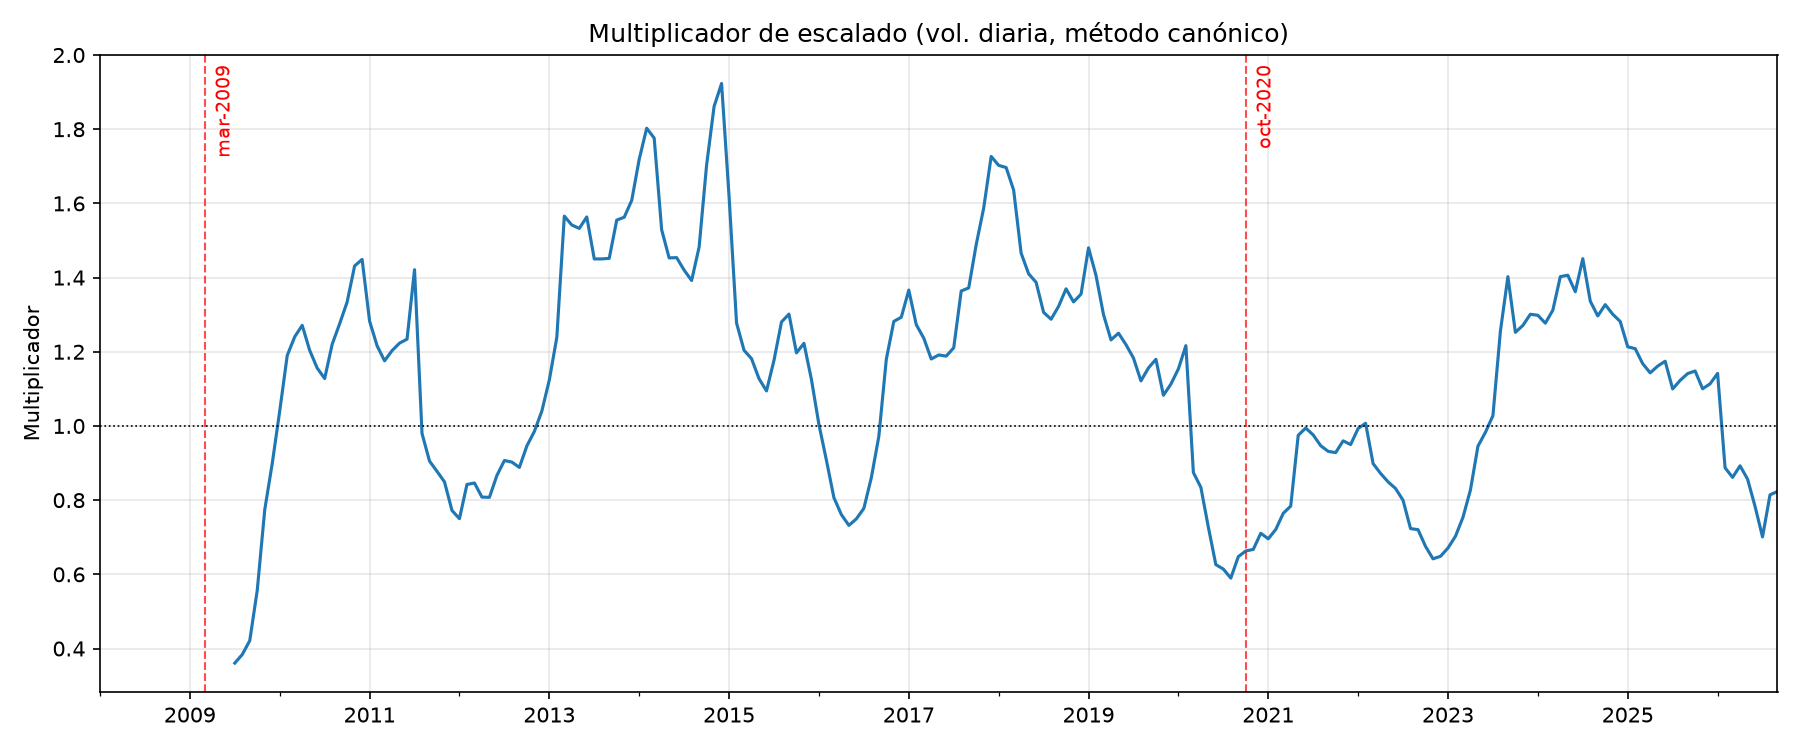
\includegraphics[width=0.9\textwidth]{fig_multiplicador.png}
\caption{Multiplicador de escalado por volatilidad (estimación diaria canónica) a lo largo de la muestra}
\label{fig:multiplicador}
\end{figure}

\section{Comparación pura vs. escalada, bruta y neta de costes}

La Tabla \ref{tab:comparativa-central} presenta la comparación central del trabajo. La columna ``pura recortada'' restringe la serie pura al mismo rango de fechas que la escalada (que pierde los primeros meses por el \textit{warm-up} de la ventana de estimación), para aislar el efecto del escalado del efecto de un periodo muestral distinto.

\begin{table}[H]
\centering
\caption{Comparación pura vs. escalada, bruta y neta de costes}
\label{tab:comparativa-central}
\resizebox{\textwidth}{!}{%
\begin{tabular}{|l|r|r|r|r|r|}
\hline
\textbf{Métrica} & \textbf{Pura bruta} & \textbf{Pura neta} & \textbf{Pura recortada (bruta)} & \textbf{Escalada bruta} & \textbf{Escalada neta} \\
\hline
Retorno anualizado & $2{,}16\%$ & $0{,}70\%$ & $3{,}64\%$ & $4{,}45\%$ & $2{,}32\%$ \\
Volatilidad anualizada & $10{,}74\%$ & $10{,}73\%$ & $9{,}63\%$ & $10{,}30\%$ & $10{,}31\%$ \\
Sharpe ratio & $0{,}201$ & $0{,}065$ & $0{,}377$ & $0{,}432$ & $0{,}225$ \\
Sortino ratio & $0{,}240$ & $0{,}078$ & $0{,}552$ & $0{,}662$ & $0{,}339$ \\
Máximo \textit{drawdown} & $-29{,}42\%$ & $-36{,}41\%$ & $-28{,}14\%$ & $-23{,}51\%$ & $-30{,}74\%$ \\
Calmar ratio & $0{,}074$ & $0{,}019$ & $0{,}129$ & $0{,}189$ & $0{,}076$ \\
Asimetría & $-1{,}338$ & $-1{,}332$ & $-0{,}428$ & $-0{,}288$ & $-0{,}299$ \\
Curtosis (Pearson) & $8{,}605$ & $8{,}637$ & $3{,}376$ & $3{,}588$ & $3{,}604$ \\
Turnover medio mensual & $0{,}772$ & $0{,}772$ & -- & $0{,}942$ & $0{,}942$ \\
Coste medio anual (pp) & $0$ & $1{,}46$ & -- & $0$ & $2{,}12$ \\
\hline
\end{tabular}%
}
\end{table}

La lectura conjunta de la Tabla \ref{tab:comparativa-central} es la siguiente. Bruto y sin ajustar por periodo muestral, el escalado casi duplica el Sharpe ($0{,}201 \rightarrow 0{,}432$, $+115\%$) --una réplica aparentemente limpia del resultado de Barroso y Santa-Clara--. Pero la serie escalada no cubre marzo de 2009 (el mes más negativo de toda la pura) por el \textit{warm-up} de la estimación de volatilidad, así que parte de esa mejora es un artefacto del periodo muestral. Comparando en igualdad de condiciones (escalada frente a pura recortada al mismo rango de fechas), la mejora de Sharpe se modera a $+15\%$ ($0{,}432$ frente a $0{,}377$) y la de Sortino a $+20\%$; la mejora de asimetría y curtosis es clara y consistente en ambas comparaciones.

Neto de costes, la ventaja de la escalada sobre la pura se mantiene ($0{,}065 \rightarrow 0{,}225$ de Sharpe), pero se reduce sustancialmente en términos absolutos: comparada contra la pura \textbf{bruta} --que ni siquiera ha pagado nada todavía--, el Sharpe neto de la escalada ($0{,}225$) apenas supera en un $12\%$ al bruto de la pura ($0{,}201$). El máximo \textit{drawdown} neto de la escalada ($-30{,}74\%$) empeora hasta quedar peor que el de la pura bruta ($-29{,}42\%$): la mejora de cola que parecía el resultado más sólido de la comparación bruta se diluye casi por completo con costes reales.

El coste medio anual de la escalada ($2{,}12$ puntos porcentuales) resultó dominado por el turnover ($1{,}84$ pp), no por la financiación del apalancamiento variable ($0{,}28$ pp) --un hallazgo que invertía la expectativa de partida--: reescalar la exposición mes a mes genera casi tanta rotación de cartera como la propia rotación de terciles del momentum (turnover medio $0{,}942$ frente a $0{,}772$ de la pura).

La Figura \ref{fig:valor-liquidativo} muestra las cuatro curvas de valor liquidativo acumulado. Se aprecia visualmente cómo la curva neta de la escalada (roja) converge hacia la pura bruta (azul) en niveles hacia el final de la muestra, mientras que la pura neta (naranja) queda claramente rezagada.

\begin{figure}[H]
\centering
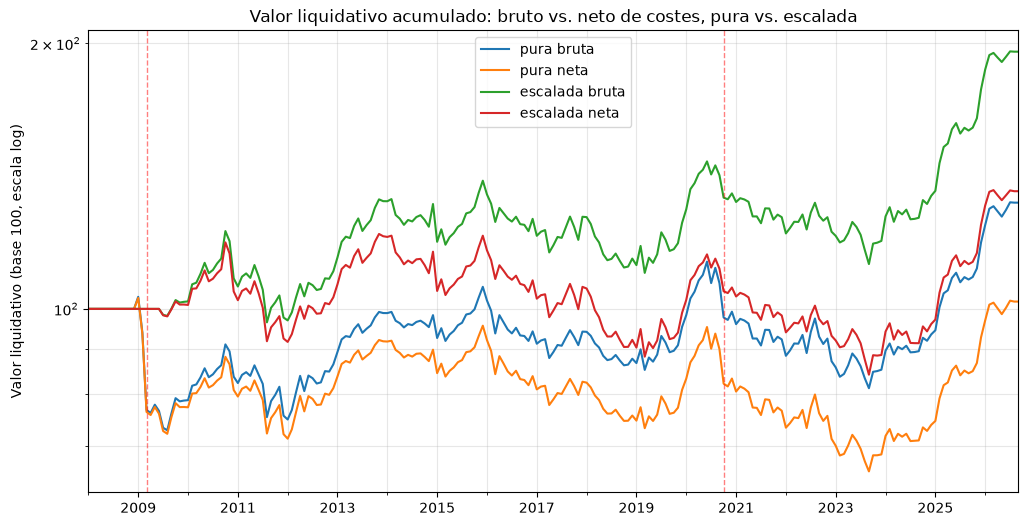
\includegraphics[width=0.9\textwidth]{fig_valor_liquidativo.png}
\caption{Valor liquidativo acumulado: pura y escalada, bruto y neto de costes (base 100, escala logarítmica)}
\label{fig:valor-liquidativo}
\end{figure}

\section{Tests de robustez}

\textbf{Bandas de no-operación.} Una banda de $\pm15\%$ sobre el multiplicador de escalado redujo el número de meses con retrade de 206 a 41, pero el turnover medio apenas bajó ($0{,}942 \rightarrow 0{,}919$, $-2{,}4\%$) y el Sharpe neto empeoró ligeramente ($0{,}225 \rightarrow 0{,}214$). La razón es mecánica: el turnover de la cartera escalada depende tanto del cambio del multiplicador como del cambio de composición de los terciles, y esta segunda fuente --que no se ve afectada por la banda-- explicaba ya el $82\%$ del turnover total. Las bandas de no-operación, tal como se plantearon, no resuelven el problema de coste identificado.

\textbf{Sensibilidad a costes.} La Figura \ref{fig:sensibilidad-costes} muestra el Sharpe neto de ambas series para un rango de $0$ a $30$ puntos básicos de coste combinado (\textit{spread} + comisión). El orden relativo (escalada por encima de pura) se mantiene en todo el rango sin cruzarse; la pura cruza a Sharpe negativo en torno a los $22$ puntos básicos, mientras que la escalada se mantiene positiva incluso en el escenario más pesimista ($0{,}046$ a $30$ pb, frente a $0{,}345$ a $5$ pb).

\begin{figure}[H]
\centering
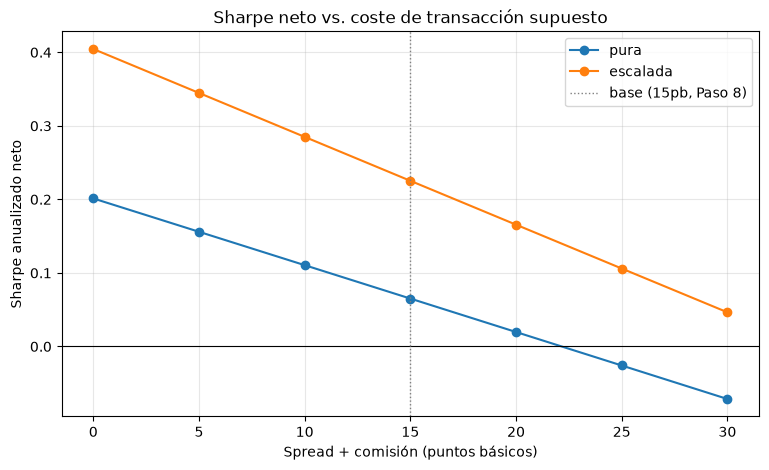
\includegraphics[width=0.8\textwidth]{fig_sensibilidad_costes.png}
\caption{Sharpe ratio neto en función del coste de transacción supuesto}
\label{fig:sensibilidad-costes}
\end{figure}

\textbf{Ventana de formación y frecuencia de rebalanceo.} La Tabla \ref{tab:sensibilidad-especificacion} muestra que la especificación 12-1 no fue una elección afortunada casual: es la de mejor resultado de las tres ventanas de formación probadas, y la única con una ventaja clara de la escalada sobre la pura. El rebalanceo trimestral reduce el turnover a la mitad en ambas series y mejora el Sharpe neto de la pura (al ahorrar más coste del que cuesta operar con una señal algo más vieja), mientras que para la escalada el efecto es neutro.

\begin{table}[H]
\centering
\caption{Sensibilidad a la ventana de formación y a la frecuencia de rebalanceo (Sharpe neto)}
\label{tab:sensibilidad-especificacion}
\begin{tabular}{|l|r|r|}
\hline
\textbf{Especificación} & \textbf{Pura} & \textbf{Escalada} \\
\hline
Formación 6-1 & $-0{,}347$ & $-0{,}449$ \\
Formación 9-1 & $0{,}039$ & $0{,}057$ \\
Formación 12-1 (base) & $0{,}065$ & $0{,}225$ \\
\hline
Rebalanceo mensual (base) & $0{,}065$ & $0{,}225$ \\
Rebalanceo trimestral & $0{,}089$ & $0{,}217$ \\
\hline
\end{tabular}
\end{table}

\textbf{Robustez por sub-periodo.} La Tabla \ref{tab:sub-periodos-etf} contiene el hallazgo más importante de esta sección: la ventaja de la escalada \textbf{no es consistente} entre sub-periodos. Está muy concentrada en 2009-2014 --precisamente el tramo en el que la escalada, por el \textit{warm-up} ya descrito, evita por construcción el crash de marzo de 2009 que sí golpea de lleno a la pura--; es prácticamente nula (de hecho, ligeramente negativa) en 2015-2020, con ambas series en Sharpe negativo; y es modesta en 2021-2026.

\begin{table}[H]
\centering
\caption{Sharpe ratio neto por sub-periodo}
\label{tab:sub-periodos-etf}
\begin{tabular}{|l|r|r|r|}
\hline
\textbf{Periodo} & \textbf{Pura} & \textbf{Escalada} & \textbf{Ventaja (escalada $-$ pura)} \\
\hline
2009-2014 & $-0{,}076$ & $0{,}316$ & $+0{,}392$ \\
2015-2020 & $-0{,}077$ & $-0{,}088$ & $-0{,}011$ \\
2021-2026 & $0{,}419$ & $0{,}504$ & $+0{,}085$ \\
\hline
\end{tabular}
\end{table}

\section{Validación externa: factor Europe Momentum (Kenneth French)}

Para determinar si la falta de consistencia por sub-periodo es un problema del mecanismo o del universo de 19 ETFs, se replicó el mismo escalado por volatilidad diaria sobre el factor \textit{Europe Momentum} (WML) de la librería de datos de Kenneth French, en bruto (sin costes, al no disponer de datos de turnover reales sobre ese factor). La Tabla \ref{tab:french-completo} muestra el resultado sobre la muestra completa (1990-2026): el escalado prácticamente duplica el Sharpe, con una mejora de asimetría y curtosis todavía más marcada que en los ETFs.

\begin{table}[H]
\centering
\caption{Factor Europe Momentum (French), muestra completa 1990-2026, bruto}
\label{tab:french-completo}
\begin{tabular}{|l|r|r|}
\hline
\textbf{Métrica} & \textbf{Pura} & \textbf{Escalada} \\
\hline
Retorno anualizado & $10{,}34\%$ & $23{,}50\%$ \\
Volatilidad anualizada & $13{,}18\%$ & $15{,}79\%$ \\
Sharpe ratio & $0{,}784$ & $1{,}489$ \\
Sortino ratio & $0{,}821$ & $2{,}755$ \\
Máximo \textit{drawdown} & $-45{,}59\%$ & $-26{,}71\%$ \\
Calmar ratio & $0{,}227$ & $0{,}880$ \\
Asimetría & $-1{,}366$ & $0{,}119$ \\
Curtosis (Pearson) & $11{,}247$ & $3{,}567$ \\
\hline
\end{tabular}
\end{table}

La comparación relevante para este trabajo, sin embargo, es en igualdad de condiciones con el universo de ETFs (Tabla \ref{tab:sintesis-final}): mismo rango de fechas (2009-2026) y mismo sub-periodo problemático (2015-2020), ambos en bruto para que la comparación sea justa (el factor de French no admite un cálculo de costes con base real).

\begin{table}[H]
\centering
\caption{Tabla de síntesis: grupo de control (ETFs) vs. benchmark académico (French), ambos en bruto}
\label{tab:sintesis-final}
\begin{tabular}{|l|r|r|}
\hline
\textbf{Métrica} & \textbf{ETFs (2009-2026)} & \textbf{French (2009-2026)} \\
\hline
Sharpe pura & $0{,}201$ & $0{,}565$ \\
Sharpe escalada & $0{,}432$ & $1{,}153$ \\
Mejora relativa & $+114{,}5\%$ & $+103{,}9\%$ \\
Sharpe pura (2015-2020) & $0{,}065$ & $0{,}780$ \\
Sharpe escalada (2015-2020) & $0{,}097$ & $1{,}177$ \\
Mejora relativa (2015-2020) & $+49{,}7\%$ & $+51{,}0\%$ \\
\hline
\end{tabular}
\end{table}

El resultado de la Tabla \ref{tab:sintesis-final} es el hallazgo central de la validación externa: la mejora \textbf{relativa} del escalado es notablemente parecida entre los dos universos, incluso en el sub-periodo 2015-2020 ($+49{,}7\%$ frente a $+51{,}0\%$, prácticamente idéntico). Esto contrasta con la Tabla \ref{tab:sub-periodos-etf}, que mostraba una ventaja neta nula en ese mismo tramo para los ETFs: la diferencia no es que el mecanismo deje de funcionar en 2015-2020, sino que esa tabla estaba calculada sobre series \textbf{netas de costes}, y en bruto el mecanismo sí mejora el Sharpe de los ETFs en ese periodo, en una magnitud casi calcada a la del benchmark académico. Lo que realmente distingue a los dos universos es el \textbf{nivel absoluto} de Sharpe bruto --entre $0{,}065$ y $0{,}201$ en los ETFs, frente a entre $0{,}565$ y $0{,}982$ en French, según el tramo--: un retorno bruto tan reducido no puede absorber ningún coste de transacción real sin volverse negativo, mientras que el del benchmark académico sí puede.

Sobre la hipótesis de decaimiento post-publicación de \citet{mcleanpontiff2016}: si el debilitamiento observado en los ETFs reflejara un decaimiento genuino y general del factor momentum con el tiempo, cabría esperar verlo también en el benchmark de French, cuya composición y metodología no cambian. No es lo que se observa: la mejora del escalado en los tres tramos largos de French no sigue una tendencia decreciente ($+76\%$ en 1991-2002, $+174\%$ en 2003-2014, $+44\%$ en 2015-2026) --el tramo intermedio es el de mayor mejora, no el de menor--, y el Sharpe bruto de la serie pura se mantiene relativamente alto y estable en todos los tramos ($0{,}57$ a $0{,}98$). La evidencia, por tanto, no apoya la hipótesis de decaimiento post-publicación como explicación del resultado débil en los ETFs.

\section{Tabla de síntesis final del checkpoint de sanidad}

La Tabla \ref{tab:cierre} resume, en una sola pantalla, el resultado base, el efecto de la banda de no-operación y el rango de sensibilidad a costes, como cierre de la fase de análisis sobre el universo de control.

\begin{table}[H]
\centering
\caption{Síntesis final: resultado base, banda de no-operación y rango de sensibilidad a costes}
\label{tab:cierre}
\begin{tabular}{|l|r|r|r|r|}
\hline
\textbf{Versión} & \textbf{Sharpe} & \textbf{Sortino} & \textbf{Turnover medio} & \textbf{Coste medio anual (pp)} \\
\hline
Pura bruta & $0{,}201$ & $0{,}240$ & $0{,}772$ & $0{,}00$ \\
Pura neta & $0{,}065$ & $0{,}078$ & $0{,}772$ & $1{,}46$ \\
Escalada bruta & $0{,}432$ & $0{,}662$ & $0{,}942$ & $0{,}00$ \\
Escalada neta & $0{,}225$ & $0{,}339$ & $0{,}942$ & $2{,}12$ \\
Escalada neta con banda $\pm15\%$ & $0{,}214$ & $0{,}314$ & $0{,}919$ & $2{,}09$ \\
\hline
\end{tabular}
\end{table}

Rango de sensibilidad a costes (5 a 30 puntos básicos): Sharpe neto de la escalada entre $0{,}046$ y $0{,}345$; Sharpe neto de la pura entre $-0{,}071$ y $0{,}156$. El ranking direccional (escalada por encima de pura) no se invierte en ningún escenario probado en todo este capítulo.

\chapter{Discusión y conclusiones}

\section{Discusión}

Los resultados del capítulo anterior permiten construir un hilo argumental coherente sobre la pregunta de investigación. El mecanismo de \textit{volatility targeting} de \citet{barroso2015} es robusto en \textbf{dirección} y en \textbf{magnitud relativa}: nunca se invierte --la escalada supera a la pura en todas las variaciones probadas (bandas de no-operación, costes de 0 a 30 puntos básicos, ventanas de formación de 6 a 12 meses, rebalanceo mensual o trimestral)--, y su mejora porcentual de Sharpe replica de forma casi idéntica la observada en el factor académico \textit{Europe Momentum} de Kenneth French, incluso en el sub-periodo 2015-2020 en el que, neto de costes, el universo de ETFs no mostraba ventaja alguna. Esta última comparación es la pieza central del argumento: si el mecanismo fuera el problema, no debería funcionar tampoco en un universo de cientos de acciones con casi cuarenta años de historia; y sin embargo funciona allí de forma consistente.

Lo que no se sostiene es que la mejora bruta observada en el universo de ETFs se traduzca en una ventaja económica sólida una vez incorporados costes de transacción realistas. La causa identificada no es el mecanismo de escalado, sino el \textbf{nivel absoluto} de Sharpe bruto del propio universo: 19 ETFs sectoriales, todos renta variable europea y por tanto altamente correlacionados entre sí, generan una señal momentum bruta muy inferior a la de un factor construido sobre cientos de acciones de 16 países. Un retorno bruto tan delgado no puede absorber costes reales sin que el resultado neto colapse --exactamente lo que documentan \citet{frazzini2018} a escala institucional, y lo que \citet{cederburg2020} encuentran como excepción favorable al momentum dentro de los portfolios gestionados por volatilidad: aquí, la excepción favorable se sostiene en dirección, pero queda muy debilitada por un universo demasiado pequeño para sostenerla en términos absolutos--.

Una aportación específica de este trabajo, no anticipada en el diseño inicial, es la identificación del turnover del propio reescalado --y no la financiación del apalancamiento variable, que se esperaba a priori como el coste dominante-- como el principal responsable del coste neto de la estrategia escalada: de los $2{,}12$ puntos porcentuales anuales de coste, solo $0{,}28$ corresponden a financiación, frente a $1{,}84$ de turnover. Esto apunta a que el coste identificado es, al menos en parte, una consecuencia de \textit{cómo} se implementó el rebalanceo (recalcular y aplicar el multiplicador exacto cada mes) y no una propiedad inevitable del mecanismo: las bandas de no-operación probadas aquí no lo resolvieron, porque la mayor parte del turnover procede de la rotación de composición entre terciles, no del cambio de escala en sí --pero esto no descarta que otras formas de suavizar el rebalanceo (por ejemplo, sobre la propia señal de ranking) puedan ser más efectivas, una vía que queda fuera del alcance de este trabajo--.

Por último, se probó explícitamente la hipótesis de que el resultado débil reflejase un decaimiento post-publicación del factor momentum, en la línea de \citet{mcleanpontiff2016}, y se descartó con evidencia propia: el sub-periodo de mayor mejora relativa del escalado en el benchmark de French (2003-2014) no es el más reciente, sino el intermedio, lo que resulta incompatible con una historia de decaimiento monótono en el tiempo.

\section{Conclusiones}

Este trabajo responde a la pregunta de investigación de forma matizada, no binaria. La mejora en el perfil riesgo-retorno que el \textit{volatility targeting} aporta al momentum \textbf{se mantiene en dirección} en un universo de inversión pequeño como el de los ETFs sectoriales europeos, incluso neta de costes de transacción y turnover reales, y esa dirección es consistente con la que exhibe un benchmark académico de referencia. Pero la mejora \textbf{no es lo bastante grande, en términos absolutos, como para constituir una ventaja económica robusta}: los costes reales erosionan entre la mitad y dos tercios del Sharpe bruto de ambas versiones de la estrategia, y la ventaja neta de la escalada frente a la pura sin escalar --la comparación que de verdad importa para decidir si esto es una estrategia viable-- se reduce a un margen modesto. La causa de fondo no es el mecanismo de escalado por volatilidad, sino la amplitud y la correlación del universo de activos sobre el que se aplica.

\section{Limitaciones}

Este trabajo tiene limitaciones que conviene explicitar. Primero, el universo de 19 ETFs sectoriales, además de pequeño, está compuesto por instrumentos altamente correlacionados entre sí (renta variable de un mismo continente y clase de activo), lo que constituye un test exigente para cualquier mecanismo de diversificación de riesgo de cola y limita la generalización de los resultados a universos con una estructura de correlación distinta. Segundo, el coste de financiación del apalancamiento variable se modelizó con el tipo de las operaciones principales de financiación del Banco Central Europeo como \textit{proxy}, al no conseguirse una serie histórica fiable de EURIBOR a 1 mes en el entorno de trabajo --una sustitución razonable pero explícitamente documentada, no el dato originalmente buscado--. Tercero, la validación externa frente al factor de Kenneth French no incorpora costes de transacción, al no existir datos de turnover ni de composición de cartera real para ese factor: sirve como comprobación \textbf{direccional} de que el mecanismo y la señal en bruto se comportan de forma parecida en ambos universos, pero no como una prueba de que la estrategia sería económicamente viable en un universo de cientos de acciones con los costes reales de negociarlas.

Una extensión natural de este trabajo sería repetir el mismo diseño --señal, escalado por volatilidad diaria, costes explícitos y tests de robustez-- sobre un universo con mayor amplitud y dispersión de correlaciones, como el de los criptoactivos, donde el momentum está documentado como especialmente intenso \citep{liutsyvinski2021} pero donde los costes de negociación reales están, con toda probabilidad, mucho menos acotados que en un ETF UCITS líquido.




%----------
%	BIBLIOGRAFÍA
%----------

%\nocite{*} % Si quieres que aparezcan en la bibliografía todos los documentos que la componen (también los que no estén citados en el texto) descomenta está línea

\clearpage
\addcontentsline{toc}{chapter}{Bibliografía}
\setquotestyle[english]{british} % Cambiamos el tipo de cita porque en el estilo IEEE se usan las comillas inglesas.
\printbibliography



%----------
%	ANEXOS
%----------

% Si tu trabajo incluye anexos, puedes descomentar las siguientes líneas
%\chapter* {Anexo x}
%\pagenumbering{gobble} % Las páginas de los anexos no se numeran



\end{document}
